\documentclass[a4paper,12pt]{article}
\usepackage{czech}                    
\usepackage[utf8]{inputenc}         
\usepackage{a4wide}                   
\usepackage[dvipdfm]{graphicx}        
\usepackage{graphics}
\usepackage{indentfirst}   
\usepackage{fancyhdr}                 
\usepackage{setspace}
\usepackage{amsmath}
\usepackage{amssymb}
\usepackage{epsfig}

%%\usepackage{nopageno}
%%\usepackage{txfonts}
\usepackage[usenames]{color}

\begin{document}
% \input epsf 
\section{Úkol}
\noindent
\begin{enumerate}
	\item Změřte tuhost aparatuty $\kappa$.
	\item Proveďte dynamickou zkošku deformace v tlaku přiloženého vzorku.
	\item Výsledek dynamické zkoušky v tlaku graficky znázorněte a určete mezní napětí $\sigma_{0.2}$ a $\sigma_U$
\end{enumerate}

\section{Teorie}
\noindent
Deformace v tlaku je případ, kdy působíme na zkoumané těleso silou $F$, která má 
nulové tečné složky. V našem případě se jedná o sílu působící kolmo na podstavy 
válečku. Tato síla způsobí, že se původní délka $l_0$ válečku zmenší na $l$ a jeho 
průměr $d_0$ se naopak zvětší na $d$. Pro popis této změny se zavádí napětí definované vztahem
\begin{eqnarray}
	\sigma={F \over S}, 
\end{eqnarray}
kde $F$ je síla popsaná výše a $S$ průřez válečku. Rozlišujeme dva základní druhy, 
a to smluvní napětí $\sigma$, kde bereme $S$ konstantní během celé deformace, a 
skutečné napětí $\sigma'$, které počítá se změnou průřetu během deformace.

Dále zavádíme relativní deformace
\begin{eqnarray}
	\varepsilon_0={l-l_0 \over l_0}={l \over l_0}-1
\end{eqnarray}
a skutečná deformace
\begin{eqnarray}
	\varepsilon=\ln{l \over l_0}
\end{eqnarray}

Dále pokud předpokládáme, že ma zkoumaný vzorek konstantní objem, tzn. nedochází 
k paltické deformaci, můžeme vyjádřit skutečné napětí
\begin{eqnarray}
	\sigma'=\sigma (1+\varepsilon_0)
\end{eqnarray}

Povrchové napětí nobývá dvou význačných hodnot. První je $\sigma_U$, kterým se 
značí mezní napětí. Do tohoto bodu se totiž látka chová dle Hookova zákonu
\begin{eqnarray}
	\sigma=\varepsilon E,
\end{eqnarray} 
kde $\varepsilon$ je relativní prodloužení a $E$ Joungův modul pružnosti v tahu 
resp. tlaku. Druhá hodnota je mez pružnosti $\sigma_E$. Po přesáhnutí toho bodu 
se stává deformace nevratnou a pokud se výrazně změní deformace, nastává takzvaný 
kluz, díky čemuž je snažší učit její hodnotu.

Zkoumaný objekt dále charakterizuje \emph{mez 0.2}, která značí napětí, při kterém 
je platcká deformace rovna 0.2 \%. Tato hodnota se dá vyčíst ze zatěžovacího diagramu. 
Za předpokladu, že platí vztah
\begin{eqnarray}
	|\varepsilon_0|=|\varepsilon_{el}|+|\varepsilon_{pl}|,
\end{eqnarray}
kde $\varepsilon_{el}$ značí eastickou složku deformace a $\varepsilon_{pl}$ složku 
plastickou, můžeme počítat s tím, že elastická složka splňuje Hookův zákon i za 
mezním napětím. Díky tomu stačí do zatěžovacího diagramu zanést přímku s předpisem 
\begin{eqnarray}
	\sigma=E(\varepsilon-0.2),
\end{eqnarray}
kde $E$ určíme z hodnot do mezního napětí. Tato přímka se nám protne s křivkou 
diagramu a v tomto bodě odečteme $\sigma_{0.2}$. 

Podrobnější popis chování tuhých látek při deformaci a přesnější modely naleznete v \cite{2}.

V našem případě rovnoměrně zvyšujeme relativní deformaci dle vztahu
\begin{eqnarray}
	\varepsilon={tvs \over l_0},
\end{eqnarray}
kde $t$ je čas, $v$ rychlost otáčení šroubu aparatury, jejíž hodnota je 
$v=0.6\cdot10^{-3}\mbox{s}^{-1}$, $s$ vzdálenost, o kterou se posune píst za 
jednu otáčku, která je $s=0.75$ mm a $l_0$ původní délka vzorku. Sílu určujeme 
díky tenzometrickému odporovému snímači, který převádí sílu na něj působící na 
napětí. Zpětně získáme sílu
\begin{eqnarray}
	F=\alpha U,
\end{eqnarray} 
kde $\alpha=50$ N/mV a $U$ je naměřené napětí.

Nakonec musíme započítat opravu na tuhost aparatury, protože se působením síly 
sama deformuje. Tuto deformaci považujeme za elastickou, proto musí splňovat rovnici
\begin{eqnarray}
	F=\kappa |\Delta l|,
\end{eqnarray}
kde $\kappa$ je tuhost aparatury, kterou změříme samostatným měřením se vzorkem 
s výrazně vyšším poloměrem, který je zhotoven z tuhého materiálu (v našem případě oceli),  
a $\Delta l$ je změna délky aparatury. Vztahu (10) využijeme při korekci relativního prodloužení vzorku.

\eject
\section{Výsledky měření}
\noindent
Teplota v laboratoři byla $297.15K$  a vlhkost 26.8 \%.

Nejprve jsem si změřil rozměry vzorku. Tyto hodnoty jsou uvedeny v tabulce 1 spolu 
s určenou střední hodnotou a statistickou chybou dle \cite{4}.

$$
\begin{array}{|l|rrrrr|c|}
\hline
	l_1/\mbox{cm}&	1.005&	1.010&	1.010&	1.005&	1.005&	1.007 \pm 0.005	\\ \hline
	d_0/\mbox{mm}&	7.46&	7.47&	7.47&	7.46&	7.47&	7.47 \pm 0.01	\\ \hline
\end{array}
$$
\vglue.05in
\begin{center}
	\textbf{Tabulka 1:} Rozměry vzorku před měřením.
\end{center}


Následně jsme určil kostantu charakterizující tuhost aparatury $\kappa$. Na 
začátku měření bylo vidět, že chvilku trvá, než si aparatura sesedne se vzorkem, 
proto jsem počáteční hodnoty zanedbal. Zbylým jsem v programu Gnuplot nafitoval 
lineární křivku a její směrnice je mnou hledaná konstanta
\begin{eqnarray}
	\kappa=(1.7 \pm 0.2)\cdot 10^6 \mbox{N/m},
\end{eqnarray}
přičemž její chyba je složena z chyb rychlosti otáčení, konstanty $\alpha$ a chyby fitu.

\begin{figure}[!htb]
	% GNUPLOT: LaTeX picture with Postscript
\begingroup
  \makeatletter
  \providecommand\color[2][]{%
    \GenericError{(gnuplot) \space\space\space\@spaces}{%
      Package color not loaded in conjunction with
      terminal option `colourtext'%
    }{See the gnuplot documentation for explanation.%
    }{Either use 'blacktext' in gnuplot or load the package
      color.sty in LaTeX.}%
    \renewcommand\color[2][]{}%
  }%
  \providecommand\includegraphics[2][]{%
    \GenericError{(gnuplot) \space\space\space\@spaces}{%
      Package graphicx or graphics not loaded%
    }{See the gnuplot documentation for explanation.%
    }{The gnuplot epslatex terminal needs graphicx.sty or graphics.sty.}%
    \renewcommand\includegraphics[2][]{}%
  }%
  \providecommand\rotatebox[2]{#2}%
  \@ifundefined{ifGPcolor}{%
    \newif\ifGPcolor
    \GPcolorfalse
  }{}%
  \@ifundefined{ifGPblacktext}{%
    \newif\ifGPblacktext
    \GPblacktexttrue
  }{}%
  % define a \g@addto@macro without @ in the name:
  \let\gplgaddtomacro\g@addto@macro
  % define empty templates for all commands taking text:
  \gdef\gplbacktext{}%
  \gdef\gplfronttext{}%
  \makeatother
  \ifGPblacktext
    % no textcolor at all
    \def\colorrgb#1{}%
    \def\colorgray#1{}%
  \else
    % gray or color?
    \ifGPcolor
      \def\colorrgb#1{\color[rgb]{#1}}%
      \def\colorgray#1{\color[gray]{#1}}%
      \expandafter\def\csname LTw\endcsname{\color{white}}%
      \expandafter\def\csname LTb\endcsname{\color{black}}%
      \expandafter\def\csname LTa\endcsname{\color{black}}%
      \expandafter\def\csname LT0\endcsname{\color[rgb]{1,0,0}}%
      \expandafter\def\csname LT1\endcsname{\color[rgb]{0,1,0}}%
      \expandafter\def\csname LT2\endcsname{\color[rgb]{0,0,1}}%
      \expandafter\def\csname LT3\endcsname{\color[rgb]{1,0,1}}%
      \expandafter\def\csname LT4\endcsname{\color[rgb]{0,1,1}}%
      \expandafter\def\csname LT5\endcsname{\color[rgb]{1,1,0}}%
      \expandafter\def\csname LT6\endcsname{\color[rgb]{0,0,0}}%
      \expandafter\def\csname LT7\endcsname{\color[rgb]{1,0.3,0}}%
      \expandafter\def\csname LT8\endcsname{\color[rgb]{0.5,0.5,0.5}}%
    \else
      % gray
      \def\colorrgb#1{\color{black}}%
      \def\colorgray#1{\color[gray]{#1}}%
      \expandafter\def\csname LTw\endcsname{\color{white}}%
      \expandafter\def\csname LTb\endcsname{\color{black}}%
      \expandafter\def\csname LTa\endcsname{\color{black}}%
      \expandafter\def\csname LT0\endcsname{\color{black}}%
      \expandafter\def\csname LT1\endcsname{\color{black}}%
      \expandafter\def\csname LT2\endcsname{\color{black}}%
      \expandafter\def\csname LT3\endcsname{\color{black}}%
      \expandafter\def\csname LT4\endcsname{\color{black}}%
      \expandafter\def\csname LT5\endcsname{\color{black}}%
      \expandafter\def\csname LT6\endcsname{\color{black}}%
      \expandafter\def\csname LT7\endcsname{\color{black}}%
      \expandafter\def\csname LT8\endcsname{\color{black}}%
    \fi
  \fi
  \setlength{\unitlength}{0.0500bp}%
  \begin{picture}(11904.00,8502.00)%
    \gplgaddtomacro\gplbacktext{%
      \csname LTb\endcsname%
      \put(1078,704){\makebox(0,0)[r]{\strut{} 0}}%
      \put(1078,2488){\makebox(0,0)[r]{\strut{} 0,5}}%
      \put(1078,4273){\makebox(0,0)[r]{\strut{} 1}}%
      \put(1078,6057){\makebox(0,0)[r]{\strut{} 1,5}}%
      \put(1078,7841){\makebox(0,0)[r]{\strut{} 2}}%
      \put(1210,484){\makebox(0,0){\strut{} 0}}%
      \put(3203,484){\makebox(0,0){\strut{} 5}}%
      \put(5196,484){\makebox(0,0){\strut{} 10}}%
      \put(7189,484){\makebox(0,0){\strut{} 15}}%
      \put(9182,484){\makebox(0,0){\strut{} 20}}%
      \put(11174,484){\makebox(0,0){\strut{} 25}}%
      \put(308,4272){\rotatebox{-270}{\makebox(0,0){\strut{}\rotatebox{-90}{$\frac{U}{\mathrm{V}}$}}}}%
      \put(6391,154){\makebox(0,0){\strut{}$\frac{I}{\mathrm{mA}}$}}%
      \put(6391,8171){\makebox(0,0){\strut{}Graf 1: Z\'avislost nap\v{e}t\'i na proudu}}%
    }%
    \gplgaddtomacro\gplfronttext{%
      \csname LTb\endcsname%
      \put(10586,1482){\makebox(0,0)[r]{\strut{}$U(I)$}}%
      \csname LTb\endcsname%
      \put(10586,1196){\makebox(0,0)[r]{\strut{}$U(I)$}}%
      \csname LTb\endcsname%
      \put(10586,910){\makebox(0,0)[r]{\strut{}$T_m$}}%
    }%
    \gplbacktext
    \put(0,0){\includegraphics{graf1}}%
    \gplfronttext
  \end{picture}%
\endgroup

	\caption{Kalibrační křivka spolu s naměřenými hodnotami.}
	\label{garf1}
\end{figure}

Poté jsem do aparatury vložil vzorek. Naměřené hodnoty spolu s kalibrační křivkou 
naleznete v obrázku 1. 


\begin{figure}[!htb]
% GNUPLOT: LaTeX picture with Postscript
\begingroup
  \makeatletter
  \providecommand\color[2][]{%
    \GenericError{(gnuplot) \space\space\space\@spaces}{%
      Package color not loaded in conjunction with
      terminal option `colourtext'%
    }{See the gnuplot documentation for explanation.%
    }{Either use 'blacktext' in gnuplot or load the package
      color.sty in LaTeX.}%
    \renewcommand\color[2][]{}%
  }%
  \providecommand\includegraphics[2][]{%
    \GenericError{(gnuplot) \space\space\space\@spaces}{%
      Package graphicx or graphics not loaded%
    }{See the gnuplot documentation for explanation.%
    }{The gnuplot epslatex terminal needs graphicx.sty or graphics.sty.}%
    \renewcommand\includegraphics[2][]{}%
  }%
  \providecommand\rotatebox[2]{#2}%
  \@ifundefined{ifGPcolor}{%
    \newif\ifGPcolor
    \GPcolorfalse
  }{}%
  \@ifundefined{ifGPblacktext}{%
    \newif\ifGPblacktext
    \GPblacktexttrue
  }{}%
  % define a \g@addto@macro without @ in the name:
  \let\gplgaddtomacro\g@addto@macro
  % define empty templates for all commands taking text:
  \gdef\gplbacktext{}%
  \gdef\gplfronttext{}%
  \makeatother
  \ifGPblacktext
    % no textcolor at all
    \def\colorrgb#1{}%
    \def\colorgray#1{}%
  \else
    % gray or color?
    \ifGPcolor
      \def\colorrgb#1{\color[rgb]{#1}}%
      \def\colorgray#1{\color[gray]{#1}}%
      \expandafter\def\csname LTw\endcsname{\color{white}}%
      \expandafter\def\csname LTb\endcsname{\color{black}}%
      \expandafter\def\csname LTa\endcsname{\color{black}}%
      \expandafter\def\csname LT0\endcsname{\color[rgb]{1,0,0}}%
      \expandafter\def\csname LT1\endcsname{\color[rgb]{0,1,0}}%
      \expandafter\def\csname LT2\endcsname{\color[rgb]{0,0,1}}%
      \expandafter\def\csname LT3\endcsname{\color[rgb]{1,0,1}}%
      \expandafter\def\csname LT4\endcsname{\color[rgb]{0,1,1}}%
      \expandafter\def\csname LT5\endcsname{\color[rgb]{1,1,0}}%
      \expandafter\def\csname LT6\endcsname{\color[rgb]{0,0,0}}%
      \expandafter\def\csname LT7\endcsname{\color[rgb]{1,0.3,0}}%
      \expandafter\def\csname LT8\endcsname{\color[rgb]{0.5,0.5,0.5}}%
    \else
      % gray
      \def\colorrgb#1{\color{black}}%
      \def\colorgray#1{\color[gray]{#1}}%
      \expandafter\def\csname LTw\endcsname{\color{white}}%
      \expandafter\def\csname LTb\endcsname{\color{black}}%
      \expandafter\def\csname LTa\endcsname{\color{black}}%
      \expandafter\def\csname LT0\endcsname{\color{black}}%
      \expandafter\def\csname LT1\endcsname{\color{black}}%
      \expandafter\def\csname LT2\endcsname{\color{black}}%
      \expandafter\def\csname LT3\endcsname{\color{black}}%
      \expandafter\def\csname LT4\endcsname{\color{black}}%
      \expandafter\def\csname LT5\endcsname{\color{black}}%
      \expandafter\def\csname LT6\endcsname{\color{black}}%
      \expandafter\def\csname LT7\endcsname{\color{black}}%
      \expandafter\def\csname LT8\endcsname{\color{black}}%
    \fi
  \fi
  \setlength{\unitlength}{0.0500bp}%
  \begin{picture}(7200.00,5040.00)%
    \gplgaddtomacro\gplbacktext{%
      \csname LTb\endcsname%
      \put(1210,704){\makebox(0,0)[r]{\strut{} 0}}%
      \put(1210,1722){\makebox(0,0)[r]{\strut{} 0.05}}%
      \put(1210,2740){\makebox(0,0)[r]{\strut{} 0.1}}%
      \put(1210,3757){\makebox(0,0)[r]{\strut{} 0.15}}%
      \put(1210,4775){\makebox(0,0)[r]{\strut{} 0.2}}%
      \put(1342,484){\makebox(0,0){\strut{} 0}}%
      \put(2447,484){\makebox(0,0){\strut{} 500}}%
      \put(3553,484){\makebox(0,0){\strut{} 1000}}%
      \put(4658,484){\makebox(0,0){\strut{} 1500}}%
      \put(5764,484){\makebox(0,0){\strut{} 2000}}%
      \put(6869,484){\makebox(0,0){\strut{} 2500}}%
      \put(308,2739){\rotatebox{-270}{\makebox(0,0){\strut{}$k$}}}%
      \put(4105,154){\makebox(0,0){\strut{}$Re$}}%
    }%
    \gplgaddtomacro\gplfronttext{%
      \csname LTb\endcsname%
      \put(5882,4602){\makebox(0,0)[r]{\strut{}Trubice 1}}%
      \csname LTb\endcsname%
      \put(5882,4382){\makebox(0,0)[r]{\strut{}Trubice 2}}%
      \csname LTb\endcsname%
      \put(5882,4162){\makebox(0,0)[r]{\strut{}Trubice 3}}%
      \csname LTb\endcsname%
      \put(5882,3942){\makebox(0,0)[r]{\strut{}16/$Re$}}%
      \csname LTb\endcsname%
      \put(5882,3722){\makebox(0,0)[r]{\strut{}0.133/Re$^{1/4}$}}%
    }%
    \gplbacktext
    \put(0,0){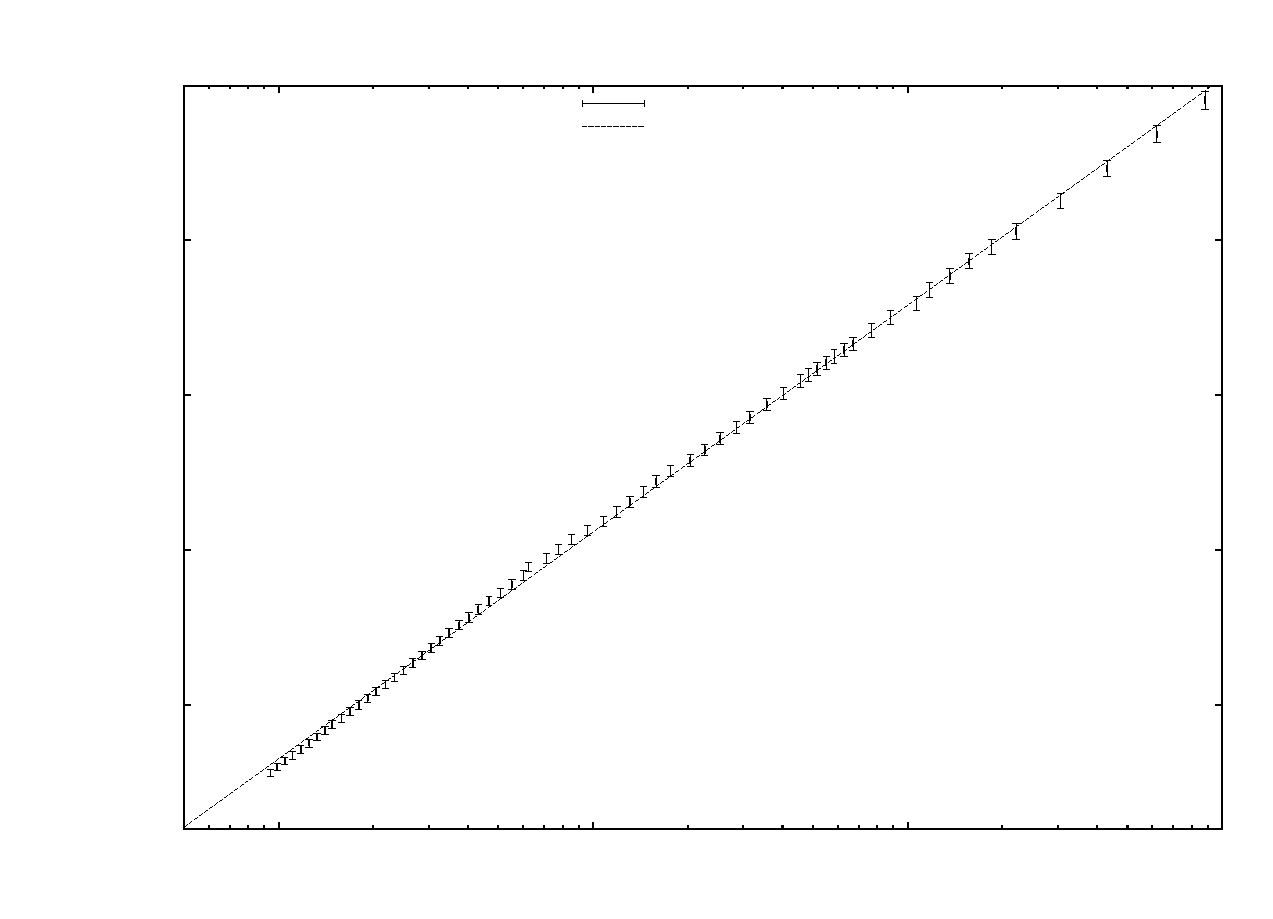
\includegraphics{graf2}}%
    \gplfronttext
  \end{picture}%
\endgroup

\caption{Výsledný graf spolu s určením $\sigma_U$ a $\sigma_{0.2}$}
\label{graf2}
\end{figure}

Následně jsem uplatnil korektury popsané výše na zanesl do grafu
křivky potřebné k určení $\sigma_U$ a $\sigma_{0.2}$. Výsledek je obrázek 2, ze kterého 
jsem odečetl hledané hodnoty a dle \cite{4} dopčetl chybu.

\begin{eqnarray}
	\sigma_{0.2}=(6.0 \pm 0.4) \mbox{MN}\cdot\mbox{m}^{-2} \\ 
	\sigma_U=(2.6 \pm 0.2) \mbox{MN}\cdot\mbox{m}^{-2}
\end{eqnarray}


Nakonec jsem přeměřil vzorek po vyjmutí z aparatury, abych se ujistil, zda došlo k elastické deformaci.
Tyto hodnoty jsou v tabulce 2.

$$
\begin{array}{|l|rrrrr|c|}
\hline
	l/\mbox{cm}&	9.970&	9.970&	9.975&	9.975&	9.975&	9.973 \pm 0.005	\\ \hline
	d/\mbox{mm}&	7.55&	7.57&	7.55&	7.56&	7.57&	7.56 \pm 0.01	\\ \hline
\end{array}
$$
\vglue.05in
\begin{center}
	\textbf{Tabulka 2:} Rozměry vzorku po měřením.
\end{center}

\section{Diskuze}
\noindent
V mém měření se vyskytla obrovská chyba způsobená mnou chybnou manipulací s aparaturou.
Markantní to je zejména na grafu 2, který neodpovídá fyzikální skutečnosti. Váleček jsem 
totiž před samotným měřením výrazně stlačil při umisťování do aparatury, z cehož vyplývá 
jistá elastická deformace na začátku měření, která není zahrnuta ve výpočtu $\varepsilon_0$.
V grafu se to projevilo vlnou za hodnotou $\sigma_U$. Z tohoto důvodu mnou určené hodnoty 
$\sigma_U$ a $\sigma_{0.2}$ nejsou příliš relevantní. Dále se při měření vyskytli drobné  
nepřesnosti. První byla nerovnoměrnost deformace vzorku. Po jeho vyjmutí z aparatury byl 
mírně prohnutý. Další chyba vznikla při kalibraci. Náš kalibrační vzorek zajisté nebyl 
dokonale tuhý a také se u  něj projevila plastická deforace. 

\section{Závěr}
\noindent
Určil jsem konstantu určující tuhost aparatury
\begin{eqnarray}
		\kappa=(1.7054 \pm 0.0007)ycdot 10^6 \mbox{N/m}.
\end{eqnarray}
Provedl jsem dynamickou zkoušku deformace vzorku, která je zobrazena v grafu 1.

\noindent
Z obrázku 2 jsem určil hodnoty
\begin{eqnarray}
	\sigma_{0.2}=(6.0 \pm 0.1) \mbox{MN}\cdot\mbox{m}^{-2}, \\ 
	\sigma_U=(2.6 \pm 0.1) \mbox{MN}\cdot\mbox{m}^{-2}.
\end{eqnarray}

\begin{thebibliography}{5}
	\bibitem{1} \textbf{Studijní text na praktikum I} \\http://physics.mff.cuni.cz/vyuka/zfp/txt\_107.pdf (21. 3. 2011)
	\bibitem{2} \emph{Prof. RNDr. Jozef Kvasnica, DrSc. a kolektiv}: \textbf{Mechanika}\\ Academia, Praha 1988
	\bibitem{4} \emph{J. Englich}: \textbf{Zpracování výsldků fyzikálních měření} \\ LS 1999/2000
\end{thebibliography}
\end{document}
